\section{Revis\~ao da Literatura}\label{sec:refteo}


Este capítulo apresenta uma revisão sistemática  da literatura nos temas relacionados a previsão de séries temporais e aplicações em hidrologia e mais especificamente em abastecimento de água. A revisão bibliográfica realizada consiste em uma análise abrangente e crítica das principais fontes de literatura. Por meio dessa revisão, busca-se obter uma compreensão aprofundada do estado atual do conhecimento na área e identificar lacunas ou oportunidades de pesquisa. As informações extraídas da literatura são fundamentais para embasar a fundamentação teórica, a metodologia e a análise dos resultados da presente dissertação.

Esta revisão sistemática da literatura (RSL) aborda o tema das séries temporais, que é relevância em diversas áreas. A seleção das referências foi baseada em critérios específicos, levando em consideração a relevância dos autores, os países com maior número de publicações e as palavras-chave mais frequentes. Também foi incluído o tema saneamento básico, que é o foco dessa dissertação.

Embora nem todos os artigos revisados tenham uma relação evidente ou mesmo acentuada aprendizado de máquina (ML), eles contribuem como material de suporte a implementação de alguns modelos avaliados para previsão este trabalho e podem servir como base para outros pesquisadores.

A Figura \ref{fig:serie-temporal} apresenta um fluxograma de como a pesquisa foi realizada, destacando a importância dos autores como base para esta revisão da literatura. 

\begin{figure}[!htb]
	\centering
	\caption{Fluxograma do problema da revisão}
	\label{fig:serie-temporal}
	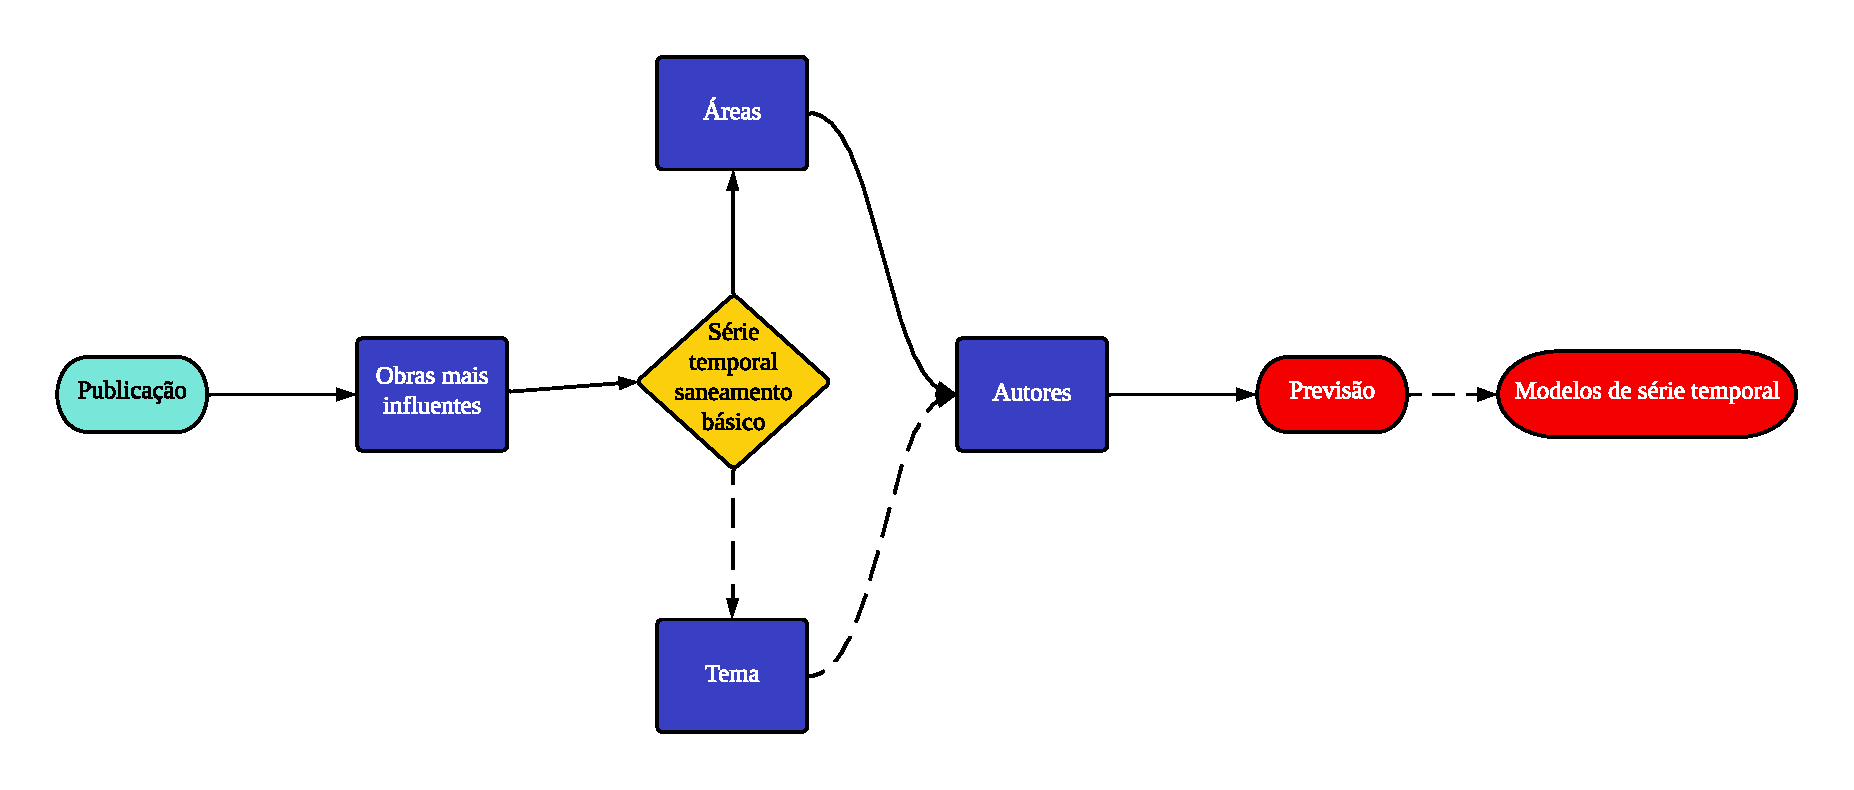
\includegraphics[width=\linewidth]{Revisao/Figuras/serie_temporal}
	
	
\end{figure}

A Figura \ref{fig:rsl} apresenta uma adaptação da metodologia proposta por \citeonline{MARTINS201671} para a realização desta RSL, foram realizadas buscas nos bancos de dados Scopus e WoS (\textit{Web of Science}), selecionando algumas bases relevantes para o tema da pesquisa.

\begin{figure}[!htb]
	\centering
	\caption{Etapas da revisão}
	\label{fig:rsl}
	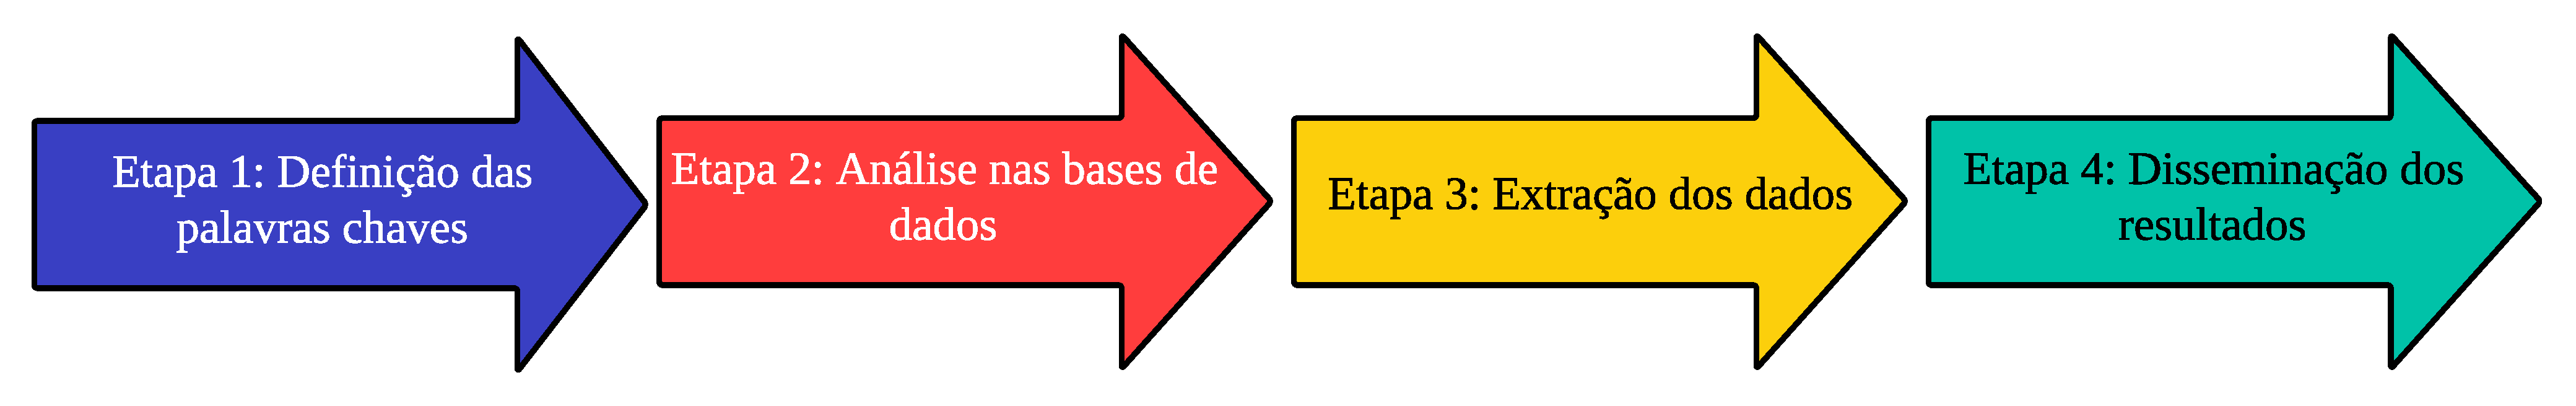
\includegraphics[width=\linewidth]{Revisao/Figuras/RSL}
	
	\fonte{Adaptado de \citeonline{MARTINS201671}}
\end{figure}

Para todas as bases de busca. Foram utilizadas palavras-chave que se adequam melhor à pesquisa, como ``\textit{time series forecasting}'', ``\textit{time series analysis}'', ``\textit{sanitation}'' e ``\textit{water supply}'' .


Na etapa seguinte, é realizada uma avaliação preliminar de cada artigo obtido, sem aplicar nenhum filtro anual nas buscas. Analisar todos os artigos dessa maneira resultaria em um número elevado, por exemplo, no banco de dados Scopus, existem 831 artigos, enquanto na WoS, são encontrados 98 artigos, totalizando 929 artigos sem a remoção de duplicatas. É importante ressaltar que esses artigos passaram apenas pelo filtro de idioma inglês e pela categoria de serem artigos, com o objetivo de aprimorar a busca e a tomada de decisões. Isso resulta em um número mais gerenciável de artigos para análise. Levando em consideração a diferença entre essa estimativa apresentada na Tabela \ref{tab:resumo} e a quantidade de artigos restantes após a remoção de duplicatas, tem-se menos de 929 artigos para análise. É válido lembrar que, ao remover as duplicatas, esse número pode diminuir ainda mais, chegando a 906 artigos, atingindo assim o objetivo proposto neste trabalho.

Na etapa final, é realizada uma análise aprofundada do conteúdo dos artigos selecionados, levando em consideração as áreas de especialização e correlação com séries temporais. Como esta revisão está inserida no contexto de um programa de mestrado em Engenharia de Produção e Sistemas, vale a pena analisar a correlação com áreas como Matemática. As áreas mais relevantes para a pesquisa são \textbf{``Informática'', ``Engenharia'' e ``Matemática''}, representando 50\% das publicações. Portanto, a pesquisa está alinhada com a utilização de conceitos matemáticos básicos para realizar uma estimativa do número de artigos.


São apresentados os resultados da pesquisa, utilizando um \textit{software} para melhor aproveitamento de cada banco de dados utilizado no trabalho. Inicialmente, é realizada uma análise no software VOSviewer.
A Figura \ref{fig:scopus-09-08} mostra os modelos que estão sendo usados com frequência, frequentemente utilizados como sinônimos ou em conjunto com ``\textit{time series}'' nos artigos. A análise da base de dados do Scopus é feita com uma ferramenta que exibe as palavras relacionadas em cada campo de busca, proporcionando uma visão abrangente das correlações com os modelos influentes.

\begin{figure}[!htb]
	\centering
	\caption{Modelos de series temporais mais populares na Scopus e WoS }
	\label{fig:scopus-09-08}
	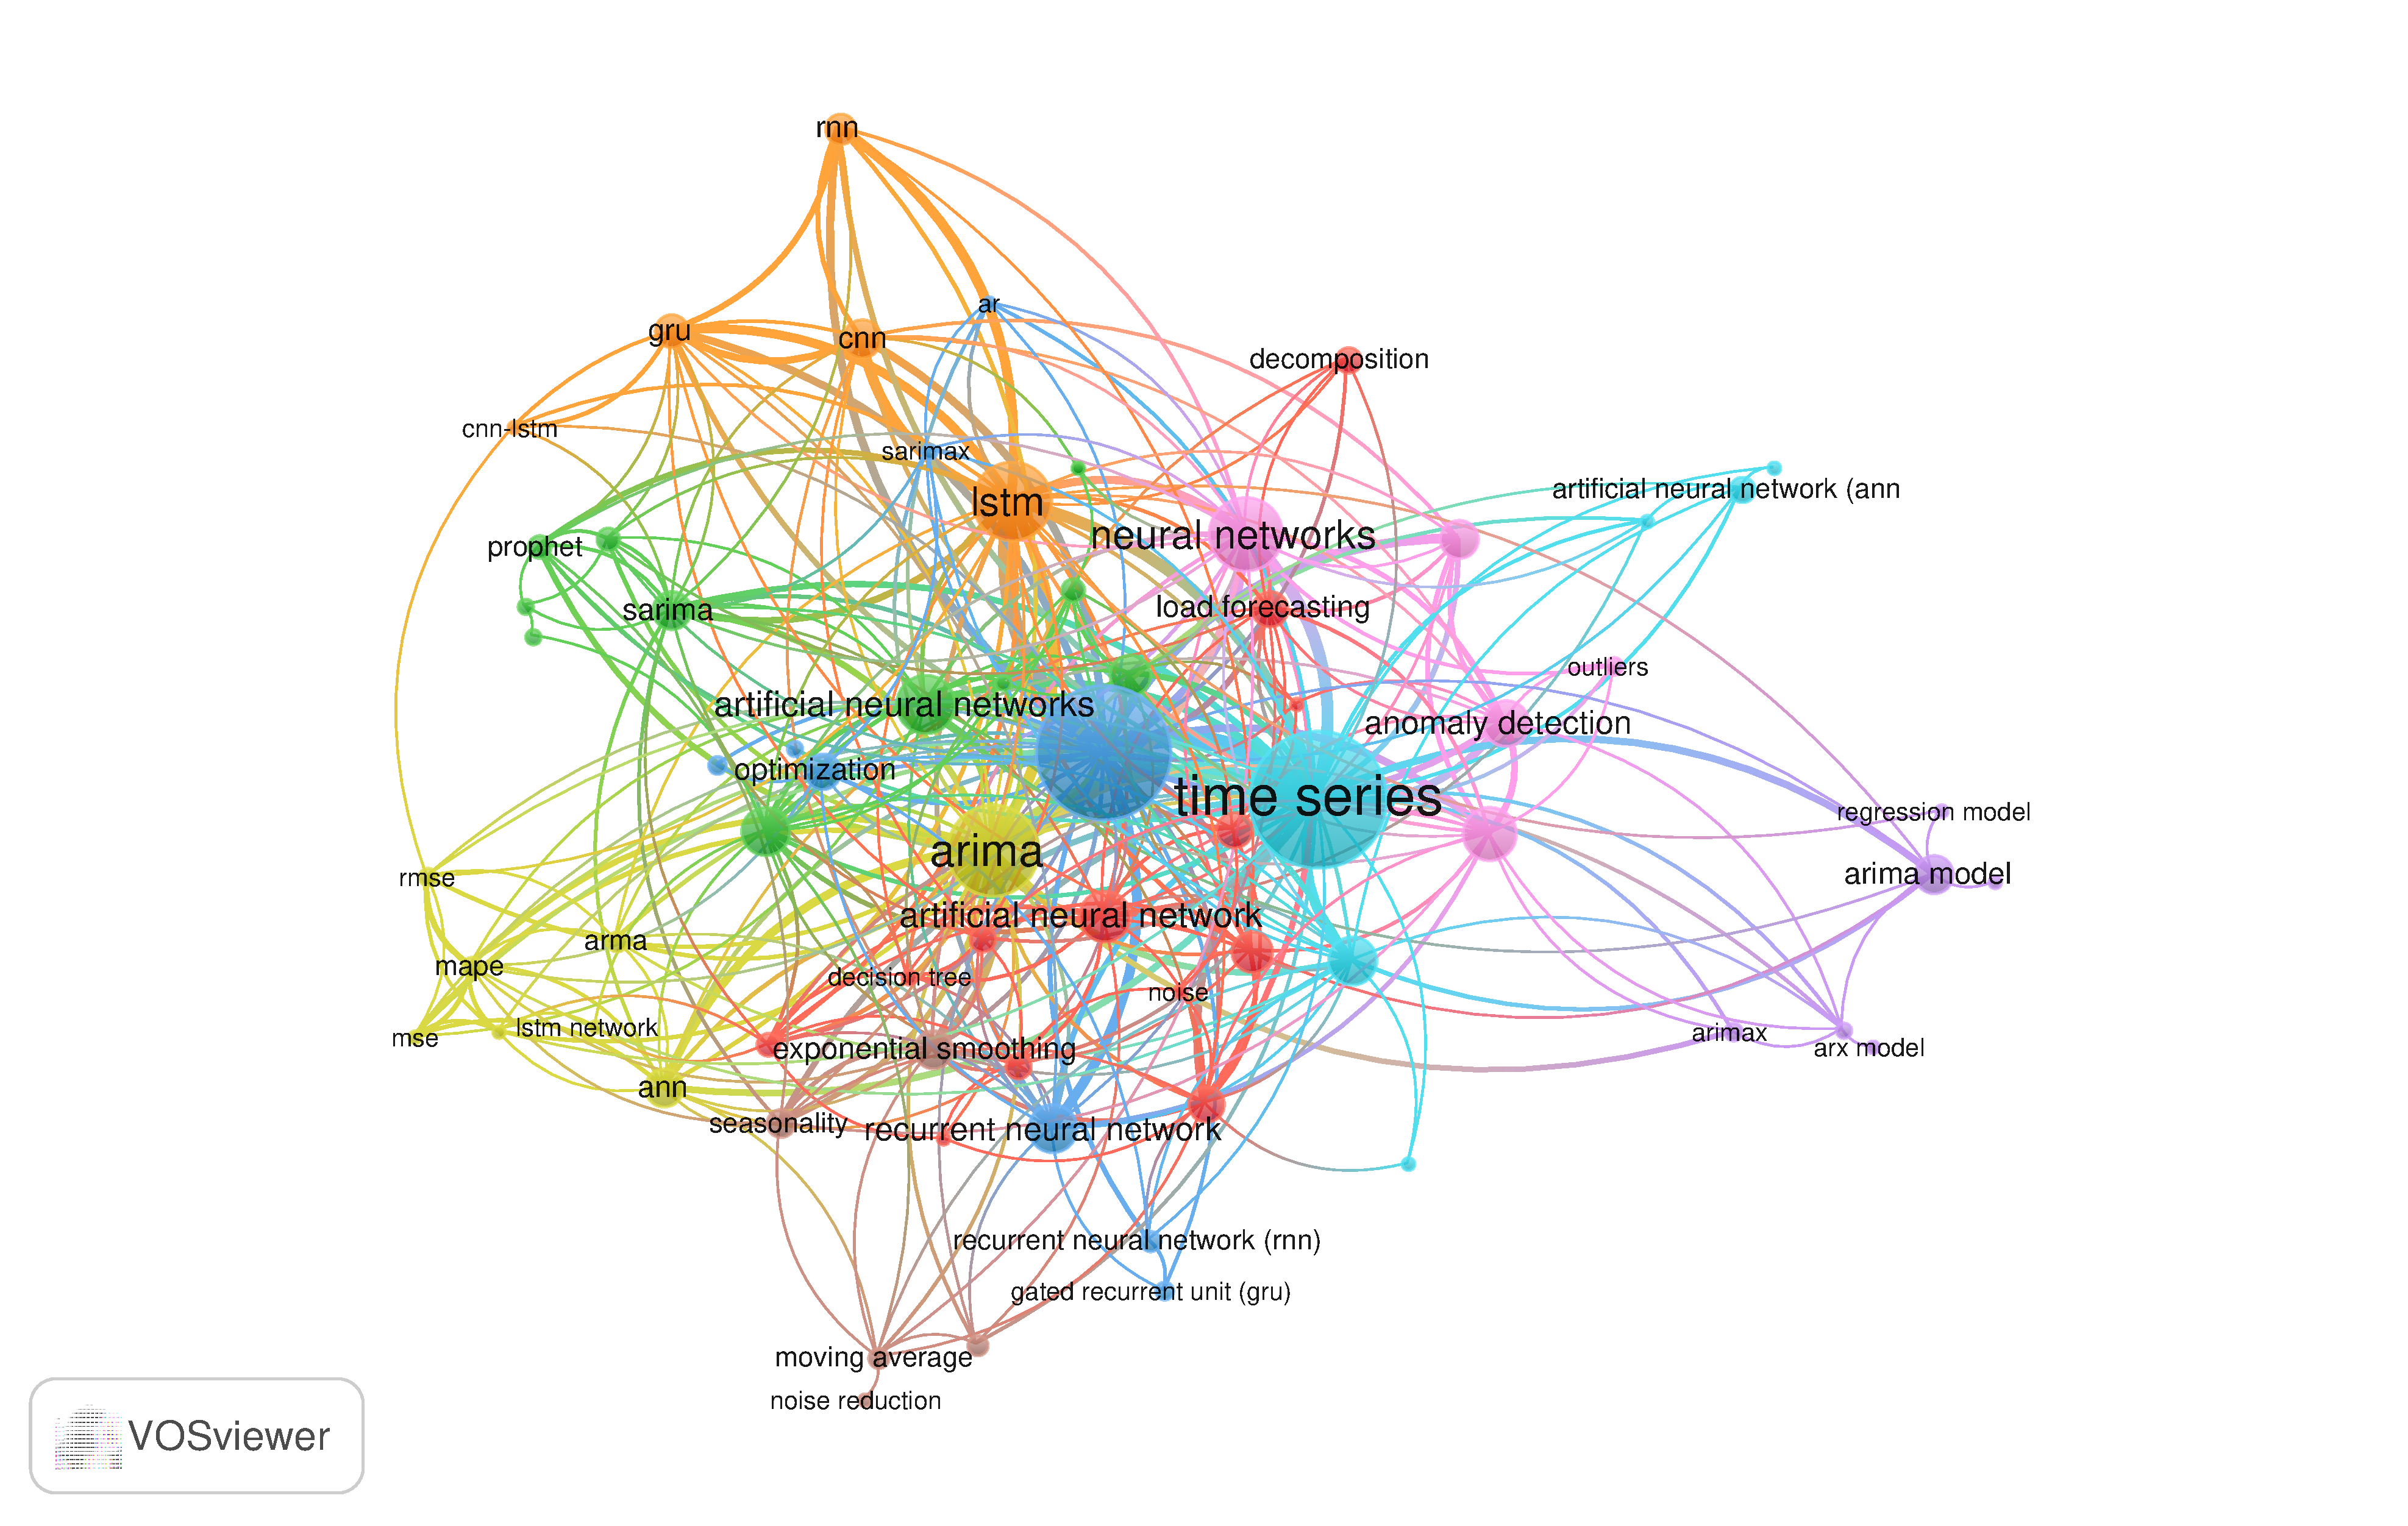
\includegraphics[width=\linewidth]{Revisao/Figuras/base-wos-scopus}
	
	
\end{figure}

Nesse primeiro momento, foram obtidos $2.555$ modelos, dos quais $83$ atingiram o limite estabelecido. É importante destacar que as palavras-chave base utilizadas são ``\textit{time series forecasting}'' ou ``\textit{time series analysis}'' e ``\textit{water supply}'' e ``\textit{sanitation}'' nas bases. Esses modelos obtidos podem estar repetidos, e é por isso que resultaram em um volume significativo de modelos.


A Tabela \ref{tb1} apresenta as palavras-chave utilizadas em cada base de dados, juntamente com o número de artigos encontrados inicialmente. No entanto, é importante ressaltar que esses dados ainda não foram processados para remover duplicatas. Após a utilização do software ScientoPy \cite{scientopy} para eliminar artigos repetidos, foram selecionados $308$ artigos únicos. Esses artigos representam a quantidade lida nesta RSL e são considerados relevantes para esta pesquisa.


\begin{table}[tb]
	\centering
	\caption{Cruzamento de palavras-chave por meio da aplicação de filtros de área}\label{tb1}
	\begin{tabular}{@{}cp{2cm}cp{2cm}cp{1.5cm}cp{2cm}c@{}}
			\toprule
			Bases                   & \multicolumn{7}{c}{Palavras chaves}                                                          & Resultados \\ \midrule
			\multirow{2}{*}{Scopus} & time series forecasting & AND & time series analysis &     &              &     &            & 798        \\
			& time series forecasting & OR  & time series analysis & AND & water supply & AND & sanitation & 33         \\
			\multirow{2}{*}{WoS}    & time series forecasting & OR  & time series analysis &     &              &     &            & 79         \\
			& time series forecasting & OR  & time series analysis & AND & water supply & AND & sanitation & 19         \\ \hline
			\multicolumn{8}{c}{Total}                                                                                              & 929        \\ \bottomrule
		\end{tabular}
	
	
\end{table}



Na Tabela \ref{tab:resumo}, os dados coletados na RSL realizada no software ScientoPy \citeonline{scientopy} são apresentados. Nessa tabela, é exibida a quantidade de artigos coletados nas bases Scopus e WoS. Apesar de um volume considerável, nem todos os artigos foram lidos integralmente, uma vez que muitos deles não se relacionavam diretamente com o objeto de pesquisa. Consequentemente, ao longo da condução da RSL, esses artigos foram excluídos.

\begin{table}[tb]
	\centering
	\caption{Resumo dos dados}
	\label{tab:resumo}
	\begin{tabular}{lc}
		\hline
		Dados Carregados & 929 \\
		Artigos Omitidos & 0 \\
		Total de Artigos & 929 \\
		Artigos da WoS & 98 \\
		Artigos do Scopus & 831 \\
		\hline
		\multicolumn{2}{c}{Remoção de Duplicados} \\
		\hline
		Porcentagem de Duplicados Encontrados & 87\% \\
		Artigos Duplicados Encontrados & 23 \\
		Contagem de Artigos Original & 929 \\
		Contagem de Artigos Atual & 906 \\
		Porcentagem de Duplicados Removidos da WoS & 19,4\% \\
		Porcentagem de Duplicados Removidos do Scopus & 0,5\% \\
		Artigos Duplicados com Diferentes Citações & 3 \\
		Porcentagem de Artigos Duplicados com Diferentes Citações & 13\% \\
		\hline
	\end{tabular}
	
	 
\end{table}


A Tabela \ref{tb2} apresenta os periódicos que mais publicaram artigos sobre o tema em questão. Todas os periódicos listadas, incluindo aquelas com um alto fator de impacto, como a categoria \textbf{Q1}, apresentam uma correlação significativa com as áreas de \textbf{informática, engenharia e matemática}.

\begin{table}[tb]
	\centering
	\caption{Fator de impacto}\label{tb2}
	\begin{tabular}{@{}cp{3cm}p{3cm}c@{}}
		\toprule
		Periódicos      & Quantidade de plubicações & Qualidade do periódico & \textit{h-index} \\\midrule
		Neurocomputing         & 27                         & Q1                     & 143     \\
		IEEE Access            & 18                         & Q1                     & 127     \\
		Applied Soft Computing & 12                         & Q1                     & 143     \\
		Energies               & 11                         & Q2                     & 93      \\
		Energy                 & 11                         & Q1                     & 343     \\ \bottomrule
	\end{tabular}
	
	
	
\end{table}

Essa observação ressalta a importância dessas áreas de especialização na pesquisa sobre séries temporais. Esses periódicos desempenham um papel fundamental na disseminação do conhecimento e no avanço do campo, garantindo a qualidade e o impacto dos artigos publicados. Portanto, é relevante direcionar a atenção para esses periódicos, uma vez que são reconhecidas como fontes confiáveis e respeitadas dentro da comunidade científica.


O ScientoPy encontra os principais tópicos de tendência com base na maior taxa de crescimento médio (AGR do inglês \textit{average growth rate}). A AGR é a diferença média entre o número de documentos publicados em um ano e o número de documentos publicados no ano anterior \cite{scientopy}. Indica como o número de documentos publicados para um tópico cresceu (número positivo) ou diminuiu (número negativo) em média dentro de um período de tempo. Este AGR é calculado utilizando a equação \eqref{arg}:


\begin{eqnarray}
	\mathrm{AGR}&=&\dfrac{\sum_{i=Y_{\mathrm{s}}}^{Y_{\mathrm{e}}} P_i-P_{i-1}}{\left(Y_{\mathrm{e}}-Y_{\mathrm{s}}\right)+1} \label{arg}
\end{eqnarray}

\noindent onde AGR $=$ taxa média de crescimento; $Y_e =$ ano final; $Y_s =$ ano inicial; $P_i =$ número de publicações no ano $i$.
Para o ano final $Y_e$, o ScientoPy utiliza o ano final global por defeito configurado nas opções globais ou/em parâmetros do comando ScientoPy. O ano de início $Y_s$ é calculado a partir do ano final $Y_e$ , conforme indicado na equação \eqref{arg2}

\begin{eqnarray}
	Y_{\mathrm{s}}&=&Y_{\mathrm{e}}-(\text { WindowWidth }+1)\label{arg2}
\end{eqnarray}

A largura da janela (do inglês \textit{Window Width}) predefinido é de 2 anos. Assim, se o ano final for 2018, o AGR é a taxa de crescimento média entre 2017 e 2018 \cite{scientopy}.

A média de documentos por ano (ADY do inglês \textit{average documents per year}) é um indicador absoluto que representa o número médio de documentos publicados num período de tempo para um tópico específico. O ADY é calculado utilizando a equação \eqref{ady}:

\begin{eqnarray}
	\mathrm{ADY}&=&\dfrac{\sum_{i={Y_{\mathrm{s}}}(t)}^{Y_{\mathrm{e}}(t)} P_i}{\left(Y_{\mathrm{e}}(t)-Y_{\mathrm{s}}(t)\right)+1}\label{ady}
\end{eqnarray}

\noindent onde $ADY$ é a média de documentos por ano; $Y_e(t)$ é o ano final; $Y_s(t)$ é o ano inicial, calculado como descrito na equação \eqref{ady}; $Pi$ é o número de publicações no ano $i$.

A percentagem de documentos nos últimos anos (PDLY do inglês \textit{Percentage of documents in last years}) é um indicador relativo que representa a percentagem do ADY em relação ao número total de documentos para um tópico específico. Desta forma, o PDLY é calculado utilizando a equação \eqref{pdly}:

\begin{eqnarray}
	\mathrm{PDLY}&=&\dfrac{\sum_{i={Y_{\mathrm{s}}(t)}}^{Y_{\mathrm{e}}(t)} P_i}{\left(Y_{\mathrm{e}(t)}-Y_{\mathrm{s}(t)}+1\right) \cdot \mathrm{TND}} \cdot 100 \%\label{pdly}
\end{eqnarray}

\noindent onde $PDLY$ é a percentagem de documentos nos últimos anos; $Y_e(t)$ é o ano final; $Y_s$ é o ano inicial, calculado como descrito na equação \eqref{pdly}; $P_i$ é número de publicações no ano i; $TND$ é o número total de documentos.

Tabela \ref{tb:autor} para visualizar de forma mais clara os autores publicou sobre o tema em análise. Essa abordagem visa evitar a inclusão de todos os autores e destacar aquele que teve uma contribuição significativa no campo. Dessa forma, é possível identificar o principal autor que se destaca nesse tópico específico, fornecendo uma visão geral da distribuição da produção científica entre os pesquisadores.

Na Tabela \ref{tb:autor} apresenta a taxa de crescimento médio (AGR), documentos médios por ano (ADY) e percentagem de documentos nos últimos anos (PDLY) período: 2021 - 2023.

\begin{table}[b]
	\centering
	\caption{Os autores que mais publicam em relação ao tema de pesquisa}\label{tb:autor}
	\begin{tabular}{ccccccc}
		\hline
		Pos & Author       & Total & AGR  & ADY  & PDLY & \textit{h-index} \\
		\hline
		1 & \citeonline{2-s2.0-84973369468} & 11 & -0.5 & 2.0 & 36.4 & 8 \\
		2 & \citeonline{2-s2.0-85123707840} & 11 & 0.0 & 3.0 & 54.5 & 5 \\
		3 & \citeonline{2-s2.0-85018469706} & 10 & 1.0 & 2.5 & 50.0 & 5 \\
		4 & \citeonline{2-s2.0-85048003524} & 9 & -1.5 & 2.0 & 44.4 & 4 \\
		5 & \citeonline{2-s2.0-84964575877} & 7 & 1.5 & 2.0 & 57.1 & 3 \\
		6 & \citeonline{2-s2.0-85063200888} & 7 & 1.0 & 2.0 & 57.1 & 3 \\
		7 & \citeonline{2-s2.0-85148656225} & 7 & 1.0 & 3.0 & 85.7 & 2 \\
		8 & \citeonline{2-s2.0-85041536076} & 7 & 1.5 & 3.0 & 85.7 & 3 \\
		9 & \citeonline{2-s2.0-85130875471} & 6 & 0.0 & 1.5 & 50.0 & 4 \\
		10 & \citeonline{2-s2.0-85061810603}& 6 & 0.0 & 1.5 & 50.0 & 5 \\
		\hline
	\end{tabular}
	
	
\end{table}


A Tabela \ref{tb:pais}, que apresenta os países com maior número de publicações sobre o tema de saneamento básico, ordenados de forma decrescente. Os principais países que se destacam nessa análise são os seguintes: China, com $179$ publicações, Estados Unidos da América com $74$ publicações, Índia com $61$ publicações, Brasil com $49$ publicações, Espanha com $40$ publicações, Reino Unido com $40$ publicações, Austrália com $31$ publicações, Itália com $26$ publicações, Canadá com $25$, Irã com $20$ publicações.

\begin{table}[tb]
	\centering
	\caption{Países com maior número de publicações}\label{tb:pais}
	\begin{tabular}{ccccccc}
		\toprule
		Pos & País & Total & AGR & ADY & PDLY & \textit{h-index} \\
		\midrule
		1 & China & 179 & 18.5 & 48.0 & 53.6 & 31 \\
		2 & Estados Unidos da América & 74 & 3.0 & 16.0 & 43.2 & 21 \\
		3 & Índia & 61 & 0.0 & 12.0 & 39.3 & 18 \\
		4 & Brasil & 49 & 3.5 & 12.5 & 51.0 & 17 \\
		5 & Espanha & 40 & 1.5 & 8.5 & 42.5 & 12 \\
		6 & Reino Unido & 40 & 3.0 & 10.0 & 50.0 & 15 \\
		7 & Austrália & 31 & 3.5 & 7.5 & 48.4 & 14 \\
		8 & Itália & 26 & 2.0 & 7.0 & 53.8 & 10 \\
		9 & Canadá & 25 & 1.0 & 5.5 & 44.0 & 11 \\
		10 & Irã & 20 & -1.0 & 3.5 & 35.0 & 11 \\
		\bottomrule
	\end{tabular}
	
	
\end{table}



Foi realizada uma investigação dos artigos na RSL. Esses artigos retratam alguns dos métodos utilizados em 
\citeonline{Taieb2016, Ursu2016, Wang2016, Graff2017, Tyralis2017, Boroojeni2017, Coelho2017, Chou2018, Bergmeir2018, Rossi2018, Ahmad2018, Chou2018a, Chen2018, Sadaei2019, Yang2019a, Buyuksahin2019, CarvalhoJr.2019, Liu2019, Shih2019a, Moon2019, Yang2019a, Xu2019, Golyandina2020, Martinovic2020a, Salgotra2020, Vlachas2020, Kulshreshtha2020, Samanta2020, Shen2020, Sezer2020, Du2020, Li2020,  Kumar2021, Lara-Benitez2021, Tan2021, Liu2021}.
Esses artigos abordam diferentes métodos usados pelos autores para previsão de séries temporais e análise não-linear dessas previsões. Eles representam contribuições significativas para o avanço do conhecimento e aplicação prática das séries temporais, sobre abordagens eficazes nesse campo. Ao incluir esses estudos influentes na análise, obtém-se uma visão abrangente dos métodos e técnicas  relevantes na previsão de séries temporais.

No estudo conduzido por \citeonline{Xu2019}, um modelo híbrido foi proposto, combinando o modelo linear AR e LR com o modelo não-linear ARIMA e o modelo DBN (do inglês \textit{Dynamic Bayesian Network}). Essa abordagem permitiu capturar tanto os comportamentos lineares quanto os não-lineares de uma série temporal. Por outro lado, \citeonline{Li2020} comparou o desempenho de previsão da abordagem MAELS (Modelo Alternativo de Estação Livre Série Temporal) com outros modelos de aprendizado de máquina de última geração, como ANN, CNN, RNN, LSTM, GRU, Transformer, Prophet, ARIMA e SVM-VAR (do inglês \textit{Support Vector Machine Variable Regression}). As abordagens ANN, CNN, RNN, GRU, Transformer e LSTM são capazes de lidar com dados multivariados de entrada e saída, enquanto o ARIMA utiliza informações passadas para prever o futuro com base em características como autocorrelação e médias móveis. Na Tabela \ref{tb:mode} é mostrado quantos artigos são relacionados em cada modelo que é utilizado neste trabalho e um artigo de cada modelo.





\begin{table}[htb]
	\centering
	\caption{Modelos baseado na literatura e nos artigos}\label{tb:mode}
	\begin{tabular}{ccccccc}
		\toprule
		Pos & Palavras-chave & Total & AGR & ADY & PDLY & \textit{h-index} \\
		\midrule
		1 & ARIMA, \citeonline{2-s2.0-85069459067} & 84 & 1.7 & 16.7 & 59.5 & 27 \\
		2 & ANN, \citeonline{2-s2.0-85054695177} & 36 & 0.7 & 9.0 & 75.0 & 17 \\
		3 & LSTM, \citeonline{WOS:000529902300014} & 35 & 3.3 & 10.7 & 91.4 & 16 \\
		4 & RNN, \citeonline{2-s2.0-85067419084} & 20 & 0.0 & 4.3 & 65.0 & 11 \\
		5 & Árvores de Decisão, \citeonline{2-s2.0-85054695177} & 12 & 0.7 & 3.0 & 75.0 & 7 \\
		6 & Transformer, \citeonline{2-s2.0-85045193200} & 10 & 2.3 & 3.0 & 90.0 & 5 \\
		7 & Random Forest, \citeonline{2-s2.0-85135210428} & 9 & 1.7 & 2.7 & 88.9 & 5 \\
		8 & CNN, \citeonline{WOS:000841076700002} & 8 & 1.3 & 2.7 & 100.0 & 4 \\
		9 & ARMA, \citeonline{2-s2.0-85038637324} & 7 & 0.3 & 0.7 & 28.6 & 6 \\
		10 & GRU, \citeonline{2-s2.0-85135210428} & 5 & 0.0 & 1.3 & 80.0 & 4 \\
		11 & SARIMA, \citeonline{2-s2.0-85128561644} & 5 & 1.0 & 1.7 & 100.0 & 4 \\
		12 & ARX, \citeonline{2-s2.0-85051469381} & 3 & 0.0 & 0.7 & 66.7 & 2 \\
		13 & LR, \citeonline{2-s2.0-85125426780} & 3 & 0.0 & 0.7 & 66.7 & 3 \\
		14 & Prophet, \citeonline{2-s2.0-85092514286} & 3 & 0.3 & 1.0 & 100.0 & 3 \\
		15 & MAPE, \citeonline{2-s2.0-85097173237} & 2 & 0.0 & 0.7 & 100.0 & 1 \\
		16 & MSE, \citeonline{2-s2.0-85096470870} & 2 & 0.0 & 0.3 & 50.0 & 2 \\
		17 & SARIMAX,\citeonline{2-s2.0-85099424908} & 2 & 0.3 & 0.7 & 100.0 & 2 \\
		18 & MAE, \citeonline{2-s2.0-85082955699} & 1 & 0.0 & 0.3 & 100.0 & 1 \\
		19 & XGBoost, \citeonline{2-s2.0-85130441623} & 1 & 0.3 & 0.3 & 100.0 & 0 \\
		\bottomrule
	\end{tabular}
	
	
	
\end{table}


Dessa forma, por meio dessa revisão sistemática e análise de conteúdo.
Além desses modelos mencionados, também será utilizada a versão atualizada do ARIMA nesta dissertação. Os modelos SARIMA e SARIMAX também serão comparados para determinar qual deles é o mais adequado. Além disso, serão empregados os modelos Light GBM e XGBoost. Os modelos de aprendizado profundo, como a RNN, ainda são considerados os melhores modelos para séries temporais no tema de saneamento básico que está sendo abordado.
Quanto a modelos, tais como RNN, CNN, ANN, LSTM, Transformer, GRU, Light GBM, XGBoost, RFR, DTR e LR, não fossem encontrados na literatura relacionados a  saneamento básico. 
Embora existam várias ramificações do modelo ARIMA, o modelo desenvolvido pelo Facebook, conhecido como Prophet, sobressai como uma opção superior em comparação com os demais. O Prophet é um modelo mais recente que simplifica significativamente muitas das tarefas que são necessárias ao lidar com o ARIMA. Enquanto o Prophet foi criado em 2017, o modelo ARIMA tem relatos de ter sido desenvolvido na década de 1960. Essa diferença temporal destaca a evolução e a modernização do campo de modelagem de séries temporais ao longo das décadas \cite{ramos2010previsoes}.











